
% Three Plans.

\section{Plans}

\subsection{The Portfolio with the minimised risk}

\begin{figure}[!h]
\centering
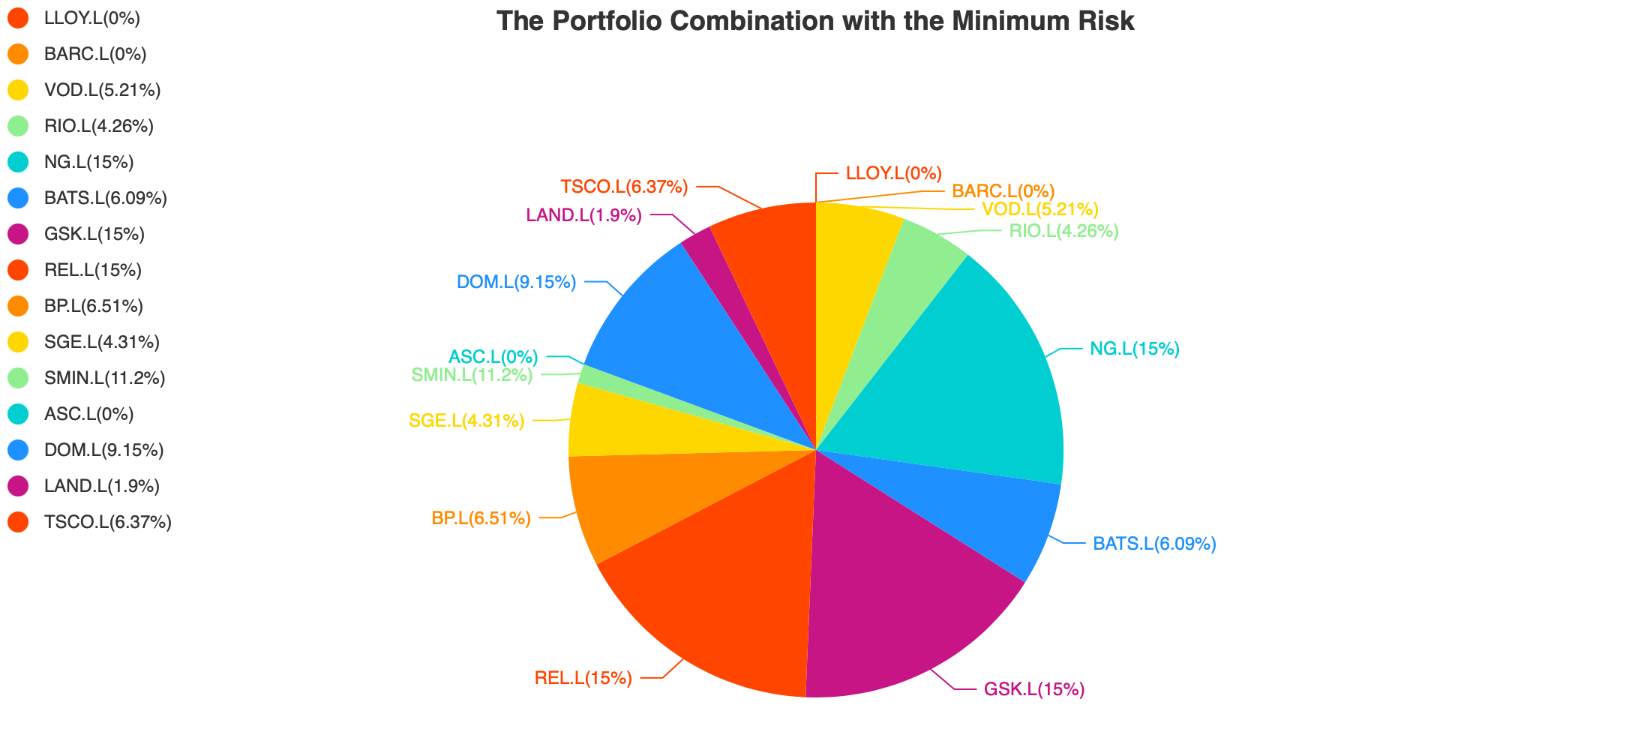
\includegraphics[width=0.9\textwidth]{minimum risk.png}
\caption{The Risk Tolerance.}
\end{figure}

%\hspace*{\fill}\\
This portfolio composed of the following stocks: \\


VOD.L(5.21\%), RIO.L(4.26\%), NG.L(15\%), BATS.L(6.09\%), GSK.L(15\%),	REL.L(15\%), BP.L(6.51\%),
SGE.L(4.31\%), SMIN.L(11.2\%), DOM.L(9.15\%), LAND.L(1.90\%), TSCO.L(6.37\%).

\newpage
    
\subsection{The portfolio with the maximised risk}
    
\begin{figure}[!h]
\centering
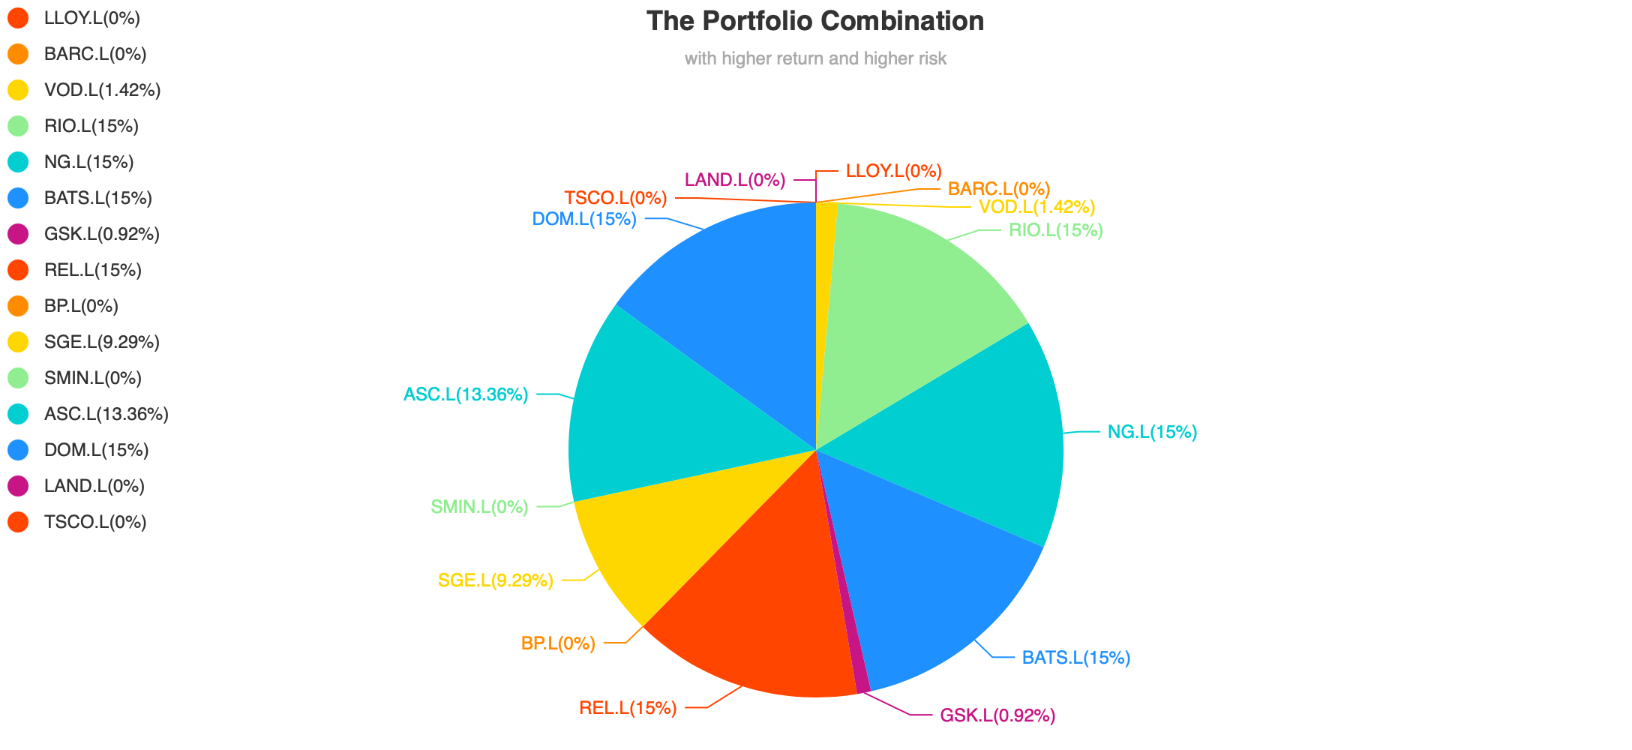
\includegraphics[width=0.9\textwidth]{higher risk.png}
\caption{The Risk Tolerance.}
\end{figure}
    
This portfolio composed of the following stocks: 
VOD.L(1.42\%), RIO.L(15\%), NG.L(15\%), BATS.L(15\%), GSK.L(0.92\%),	REL.L(15\%), SGE.L(9.29\%), ASC.L(13.36\%), DOM.L(15\%)

\newpage